\chapter{مراجعة البيانات ومعالجة الملاحظات}
\label{ch:07-review}
\section{كيف تمر الإجابة بالمراجعة؟}
\label{sec:review-flow}

الإرسال لا يعني أن البيانات صحيحة. لذلك تمر كل إجابة بمراجعين بالترتيب الذي رسمناه في القسم~\ref{sec:observatory-approval-path}: تدقيق آلي يقترح، ثم قائد الفريق، ثم مدقق المحافظة، ثم محلل الموضوع. ولا تصبح الإجابة «مقبولة» إلا بعد آخر توقيع.

يقيّم كل مراجع الإجابات واحدة واحدة، ثم يختار قراراً من ثلاثة:

\begin{table}[H]
\centering
\caption{قرارات المراجع وأثر كل منها}
\label{tab:review-decisions}
\begin{tabularx}{\linewidth}{R{3.2cm} Y Y}
\rcHeaderRow
\thh{القرار} & \thh{ما يحدث للإجابة} & \thh{متى تختاره؟}\\
«موافقة» & تنتقل إلى المرحلة التالية. وبعد آخر مرحلة تصبح «مقبول». & كل الإجابات «صحيح» أو «لا ينطبق».\\
«إعادة للتصحيح» & تعود إلى الباحث بحالة «بحاجة لاستكمال»، ومعها ملاحظاتك. & خطأ يستطيع الباحث تصحيحه.\\
«رفض» & تنتهي المراجعة، وتصبح الإجابة «مرفوض». & بيانات لا تصلح، مثل منشأة خاطئة أو تعبئة غير جادة.\\
\end{tabularx}
\end{table}

يفيدك هذا الترتيب في أمرين: لا يصل رقم إلى ملف المنشأة أو اللوحات قبل أن يراه ثلاثة أشخاص، ويعرف الباحث بالضبط ما عليه تصحيحه.

\begin{rcnote}[تطبيق المثال]
أرسل عمر في الفصل السادس «بيانات التشغيل» بسبب توقف «أخرى». ستلاحظ ليلى أن السبب غير محدد، فتعيده للتصحيح. يصححه عمر، ثم توقّع ليلى وخالد ورنا بالترتيب.
\end{rcnote}

\section{اضبط خطوة الموافقة في «المسار»}
\label{sec:review-setup}

قبل أن يراجع أحد، تبني سارة خطوة الموافقة في النموذج نفسه. افتح النموذج، ثم «المسار» من أدوات النموذج. فعّل «خطوات الموافقة»، ثم اضغط «خطوة موافقة» في شريط المسار.

\begin{figure}[H]
\centering
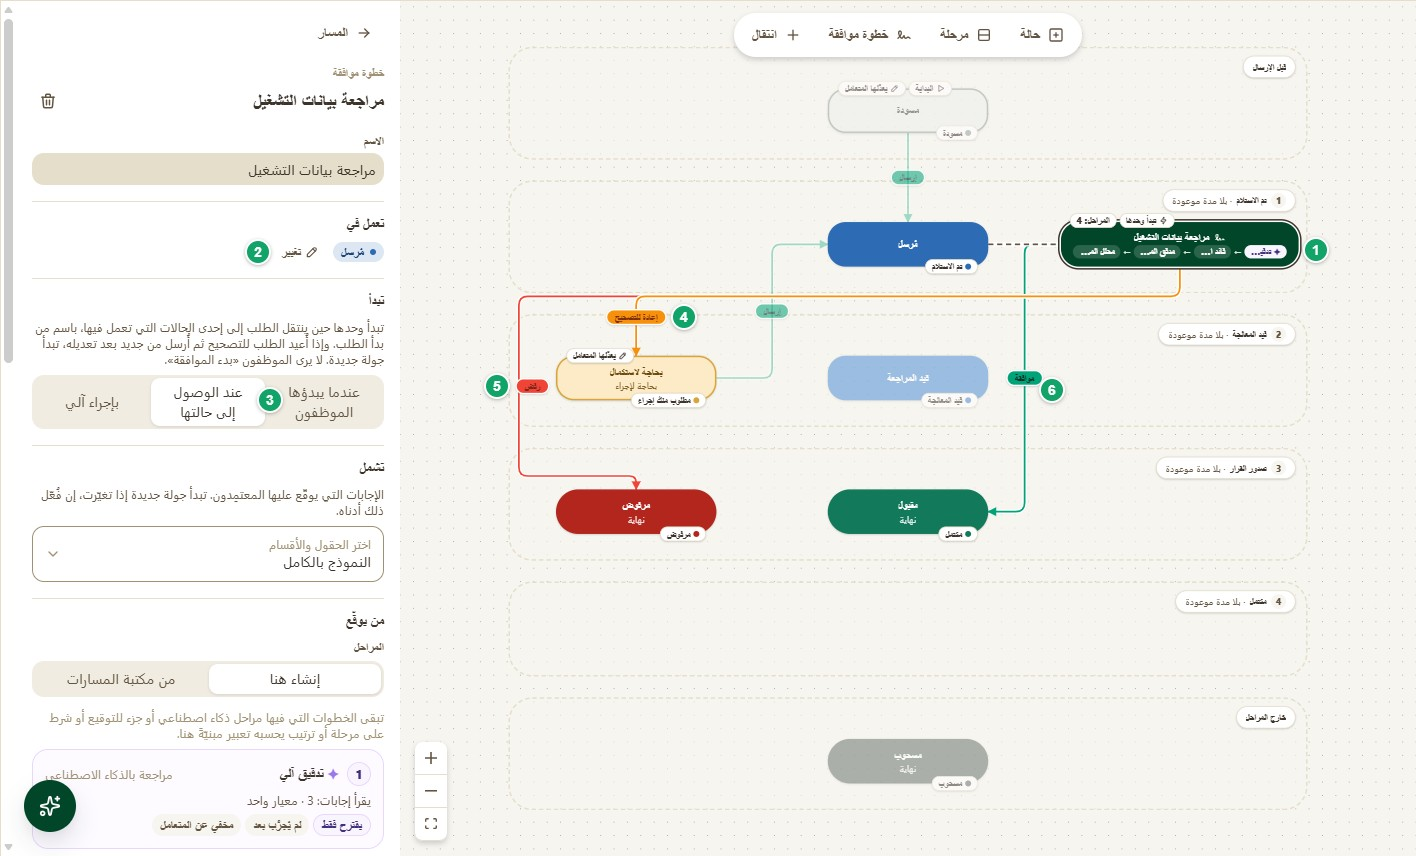
\includegraphics[width=\linewidth]{assets/screens/review-path-ar.jpg}
\caption{مسار «بيانات التشغيل» بعد إضافة خطوة الموافقة}
\label{fig:review-path}
\shotnote{يعرض المسار حالات الإجابة من «مسودة» إلى «مقبول»، والأسهم التي تنقلها بينها. وتظهر خطوة الموافقة صندوقاً أخضر في حالة «مُرسل»، تتتابع فيه مراحلها الأربع. أما الأسهم الثلاثة الخارجة منها فهي نتائج المراجعة. ① خطوة الموافقة ومراحلها. ② «تعمل في»: «مُرسل». ③ «تبدأ»: «عند الوصول إلى حالتها». ④ «إعادة للتصحيح» إلى «بحاجة لاستكمال». ⑤ «رفض» إلى «مرفوض». ⑥ «موافقة» إلى «مقبول».}
\end{figure}

\begin{figure}[H]
\centering
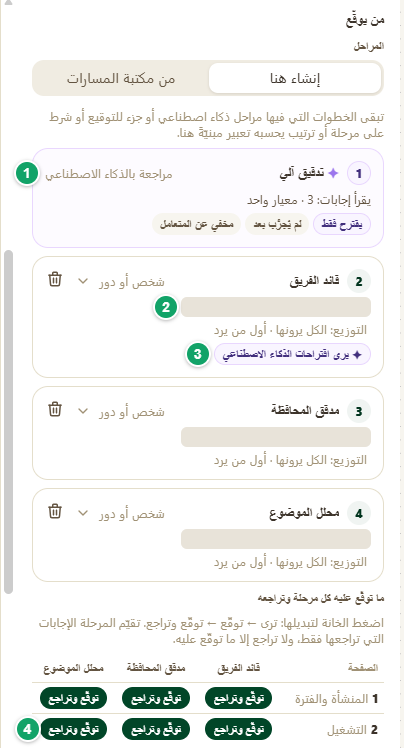
\includegraphics[width=0.62\linewidth]{assets/screens/review-stages-ar.png}
\caption{مراحل الخطوة، وما توقّع عليه كل مرحلة}
\label{fig:review-stages}
\shotnote{هنا تحدد من يوقّع وبأي ترتيب، وعلى أي صفحات. ① «تدقيق آلي»: «مراجعة بالذكاء الاصطناعي» تقرأ ثلاث إجابات بمعيار واحد، و«يقترح فقط»، وهي «مخفي عن المتعامل». ② المعتمِد: شخص أو دور، وقد أُخفي الاسم. ③ «يرى اقتراحات الذكاء الاصطناعي». ④ «توقّع وتراجع» في الصفحتين، للمراحل الثلاث.}
\end{figure}

\begin{figure}[H]
\centering
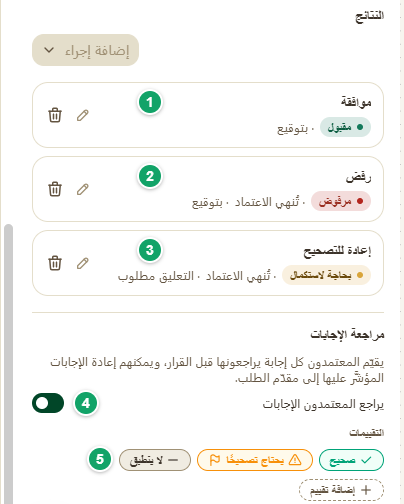
\includegraphics[width=0.62\linewidth]{assets/screens/review-results-ar.png}
\caption{نتائج الخطوة وتقييمات الإجابات}
\label{fig:review-results}
\shotnote{تحدد النتائج ما يستطيع المراجع أن يقرره، وإلى أين ينقل كل قرار الإجابة. وتحدد التقييمات ما يضعه على كل إجابة قبل القرار. ① «موافقة»: إلى «مقبول»، «بتوقيع». ② «رفض»: إلى «مرفوض»، و«تُنهي الاعتماد». ③ «إعادة للتصحيح»: إلى «بحاجة لاستكمال»، و«التعليق مطلوب». ④ «يراجع المعتمدون الإجابات». ⑤ «التقييمات»: «صحيح» و«يحتاج تصحيحًا» و«لا ينطبق».}
\end{figure}

\begin{table}[H]
\centering
\caption{حقول خطوة الموافقة}
\label{tab:review-setup-fields}
\begin{tabularx}{\linewidth}{R{3.2cm} Y Y}
\rcHeaderRow
\thh{الحقل} & \thh{ماذا يفعل؟} & \thh{الفائدة}\\
«الاسم» & اسم الخطوة كما يظهر للمراجعين. & يميّز مراجعة هذا النموذج عن غيره.\\
«تعمل في» & الحالة التي تعمل فيها الخطوة. اختر «مُرسل». & تبدأ المراجعة بعد الإرسال مباشرة.\\
«تبدأ» & «عند الوصول إلى حالتها»: تبدأ وحدها. وإذا أُعيدت الإجابة ثم أُرسلت بعد تعديلها، تبدأ جولة جديدة. & لا ينتظر أحد أن يبدأ المراجعة يدوياً.\\
«تشمل» & الإجابات التي يوقّع عليها المعتمِدون: «النموذج بالكامل»، أو حقول وأقسام تختارها. & تحدد ما يشمله التوقيع بدقة.\\
«المراحل» & «إنشاء هنا»: تضيف المراحل بالترتيب. لكل مرحلة اسم، و«شخص أو دور»، والتوزيع، مثل «الكل يرونها · أول من يرد». & ينتقل الطلب من مرحلة إلى التي تليها، فلا يرى خالد الإجابة قبل توقيع ليلى.\\
«مراجعة بالذكاء الاصطناعي» & مرحلة تقرأ إجابات تختارها، وتقارنها بمعيار تكتبه، ثم تقترح تقييماً. توضع أولاً، ولا تعتمد شيئاً. & تنبّه المراجع إلى الإجابة المشكوك فيها قبل أن يقرأها.\\
«ما توقّع عليه كل مرحلة وتراجعه» & اضغط الخانة لتبديلها: «ترى»، ثم «توقّع»، ثم «توقّع وتراجع». & تقيّم كل مرحلة الصفحات التي تخصها فقط.\\
«النتائج» & القرارات المتاحة وما تنقل إليه. أضف ما ينقص من «إضافة إجراء»، مثل «طلب تغييرات» لإعادة الإجابة. & يرى المراجع الأزرار التي يحتاجها فقط.\\
«مراجعة الإجابات» & «يراجع المعتمدون الإجابات»: يقيّم المراجع كل إجابة قبل القرار، ويعيد المؤشَّر عليها إلى الباحث. & تصل الملاحظة إلى السؤال نفسه، لا إلى النموذج كله.\\
«إعدادات أخرى» & «جولة جديدة عند التغيير». & لا يمر تعديل بعد التوقيع دون مراجعة جديدة.\\
\end{tabularx}
\end{table}

\begin{rcnote}[تنبيه: ضع الأسئلة داخل قسم]
لا تقبل الصفحة «توقّع وتراجع» إلا إذا كانت أسئلتها داخل قسم. فإذا بقيت خانة الصفحة تتبدل بين «ترى» و«توقّع» فقط، أضف قسماً في الصفحة، واسحب الأسئلة إليه، ثم عد إلى المسار.
\end{rcnote}

بعد الضبط انشر النموذج، ثم انشر الحزمة. وإذا كانت الجولة قد بدأت، فاضغط «نقل الجولة إلى الأحدث» في الخطة. أما الإجابات التي بدأت قبل ذلك فتبقى على إصدارها القديم، بلا خطوة الموافقة الجديدة.

\begin{rcnote}[تطبيق المثال]
تسمي سارة الخطوة «مراجعة بيانات التشغيل»، وتختار «مُرسل» و«عند الوصول إلى حالتها». تضيف «تدقيق آلي» بمعيار «سبب توقف محدد» على «سبب التوقف» وحده، ثم ثلاث مراحل: «قائد الفريق» لليلى، و«مدقق المحافظة» لخالد، و«محلل الموضوع» لرنا. تختار «توقّع وتراجع» للصفحتين، وتضيف «إعادة للتصحيح»، وتفعّل «يراجع المعتمدون الإجابات». وفي «متابعة الاحتياج» تبني خطوة بمرحلتين فقط: ليلى ثم رنا.
\end{rcnote}

\section{قيّم كل إجابة}
\label{sec:review-rate}

تجد ليلى الطلب في صفحتها الرئيسية، وفي «طلبات الموافقة» ثم «بانتظارك». تفتحه فترى إجابات عمر، وتحت كل إجابة تقييمها.

\begin{figure}[H]
\centering
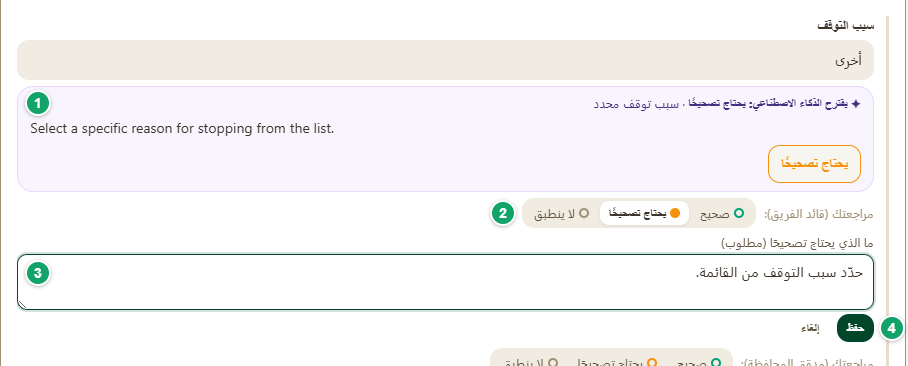
\includegraphics[width=\linewidth]{assets/screens/review-rating-ar.png}
\caption{تقييم إجابة «سبب التوقف»}
\label{fig:review-rating}
\shotnote{هذا تقييم إجابة واحدة، ويتكرر تحت كل سؤال. يفيدك في أن تحدد الخطأ في موضعه، فيعرف الباحث ما يصححه دون أن يخمّن. وقد ظهر نص الاقتراح بالإنجليزية في بيئة التجربة. ① اقتراح «تدقيق آلي»: «يحتاج تصحيحًا» مع سببه. ② «مراجعتك (قائد الفريق)»: «صحيح» أو «يحتاج تصحيحًا» أو «لا ينطبق». ③ «ما الذي يحتاج تصحيحًا (مطلوب)». ④ «حفظ».}
\end{figure}

\begin{enumerate}
\item اقرأ كل إجابة، واختر تقييمها. اقتراح الذكاء الاصطناعي مساعدة فقط؛ القرار لك.
\item عند «يحتاج تصحيحًا» اكتب ما يجب تصحيحه، ثم اضغط «حفظ». الملاحظة إلزامية.
\item تابع العداد في لوحة القرار، مثل «روجعت 5 من 5 إجابة».
\end{enumerate}

\begin{rcnote}[تطبيق المثال]
تقيّم ليلى أربع إجابات «صحيح». وفي «سبب التوقف» توافق الاقتراح الآلي: تختار «يحتاج تصحيحًا»، وتكتب «حدّد سبب التوقف من القائمة.»، ثم تضغط «حفظ».
\end{rcnote}

\section{قرّر ووقّع}
\label{sec:review-decide}

بعد التقييم تختار القرار من لوحة «سير الطلب». ويمنعك النظام من «موافقة» ما دامت هناك إجابة قيّمتها «يحتاج تصحيحًا».

\begin{figure}[H]
\centering
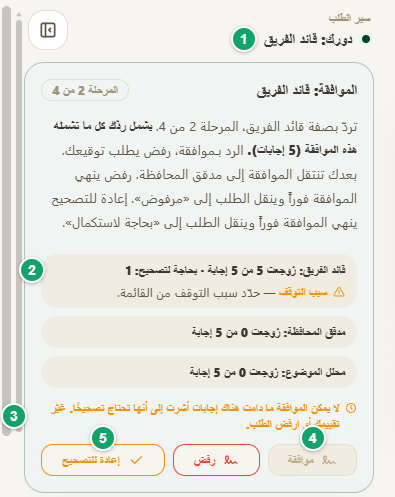
\includegraphics[width=0.62\linewidth]{assets/screens/review-decision-ar.png}
\caption{لوحة القرار وزر الموافقة معطّل}
\label{fig:review-decision}
\shotnote{تعرض اللوحة دورك في المسار، وما راجعته كل مرحلة، والقرارات المتاحة لك. تفيدك في معرفة سبب تعطل الموافقة، وأثر كل قرار قبل أن تضغطه. ① «دورك: قائد الفريق»، و«المرحلة 2 من 4». ② «روجعت 5 من 5 إجابة · بحاجة لتصحيح: 1»، والسؤال المؤشَّر عليه. ③ سبب تعطل الموافقة. ④ «موافقة»: معطّلة. ⑤ «إعادة للتصحيح»، وبجانبها «رفض».}
\end{figure}

يفتح كل قرار نافذة تأكيد، لأن القرار توقيع تتحمل مسؤوليته:

\begin{figure}[H]
\centering
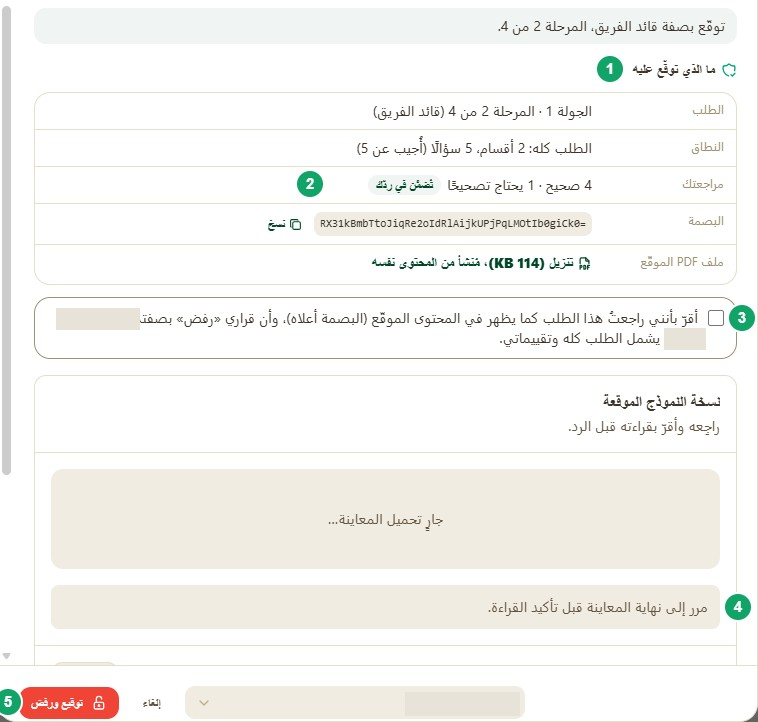
\includegraphics[width=\linewidth]{assets/screens/review-confirm-ar.jpg}
\caption{نافذة تأكيد القرار والتوقيع}
\label{fig:review-confirm}
\shotnote{تعرض النافذة ما ستوقّع عليه بالضبط قبل أن توقّع. وتظهر في الصورة لقرار «رفض»، وهي النافذة نفسها لكل قرار، ويتغير اسم الزر فقط. أُخفي الاسم في سطرين. ① «ما الذي توقّع عليه»: الجولة والمرحلة والنطاق، وبصمة المحتوى، وملف PDF الموقّع. ② «مراجعتك»: ملخص تقييماتك. ③ الإقرار بأنك راجعت الطلب. ④ «مرر إلى نهاية المعاينة قبل تأكيد القراءة.». ⑤ زر التوقيع، مثل «توقيع ورفض».}
\end{figure}

\begin{enumerate}
\item ضع علامة الإقرار.
\item مرّر نسخة النموذج الموقعة إلى نهايتها، ثم اضغط «تأكيد القراءة».
\item اكتب التعليق إذا كان مطلوباً، كما في «إعادة للتصحيح».
\item اضغط زر التوقيع. اختر ملف مفتاحك، ثم أدخل رمز PIN في «تأكيد التوقيع».
\end{enumerate}

\textbf{مفتاح التوقيع:} يحتاج كل مراجع إلى مفتاح توقيع مرة واحدة. يصدر له مسؤول المؤسسة «رمز تسجيل» من «مفاتيح الأعضاء»، وهو صالح 15 دقيقة ولمرة واحدة. ثم يفتح المراجع «إعدادات الحساب» ثم «إدارة التوقيع»، ويضغط «إنشاء توقيع». يمر بأربع خطوات: «رمز التسجيل»، و«إعداد رمز PIN»، و«تأكيد رمز PIN»، و«رسم التوقيع». وبعدها يضغط «إنشاء وتنزيل»، ويحفظ ملف المفتاح في مكان آمن. دون هذا المفتاح لا يكتمل أي توقيع.

\begin{rcnote}[تطبيق المثال]
تضغط ليلى «إعادة للتصحيح». تضع علامة الإقرار، وتؤكد القراءة، وتكتب التعليق «حدّد سبب التوقف من القائمة.»، ثم توقّع بملف مفتاحها ورمزها. تصبح الإجابة «بحاجة لاستكمال»، وتعود إلى عمر.
\end{rcnote}

\section{صحّح وأعد الإرسال}
\label{sec:review-correct}

يجد الباحث الإجابة المعادة في «التكليفات»، وعلى البطاقة الحالة «بحاجة لاستكمال». يفتحها فيرى بجانب كل إجابة تقييمها، وتحت المؤشَّر عليها ملاحظة المراجع.

\begin{figure}[H]
\centering
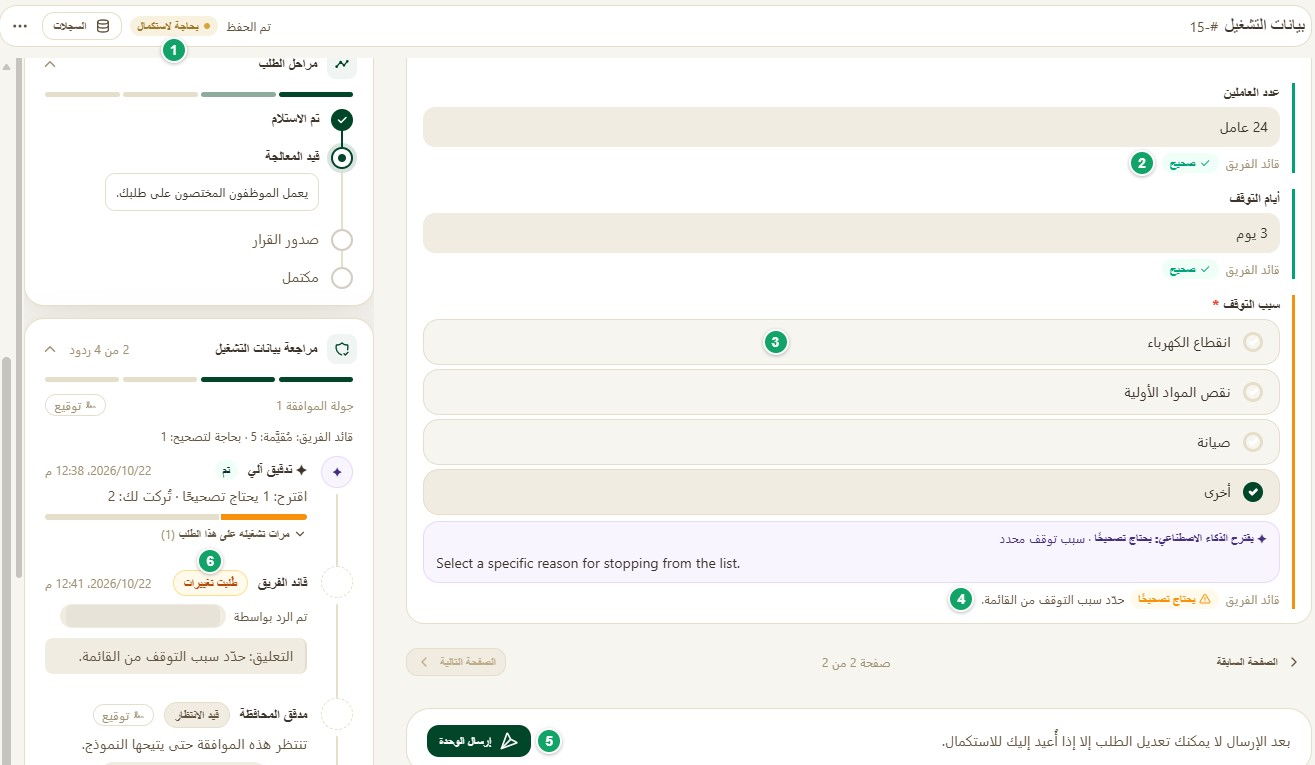
\includegraphics[width=\linewidth]{assets/screens/review-correct-ar.jpg}
\caption{الإجابة المعادة كما يراها عمر}
\label{fig:review-correct}
\shotnote{هذه الإجابة بعد إعادتها: الأسئلة المقبولة عليها «صحيح»، والمعادة عليها ملاحظة واضحة. تفيد الباحث في تصحيح المطلوب وحده، ثم الإرسال من جديد. ① «بحاجة لاستكمال». ② «صحيح» على «عدد العاملين». ③ خيارات «سبب التوقف»، وهي مفتوحة للتعديل. ④ «يحتاج تصحيحًا» وملاحظة ليلى. ⑤ «إرسال الوحدة». ⑥ «طلبت تغييرات» في سجل المراجعة، وقد أُخفي الاسم.}
\end{figure}

\begin{enumerate}
\item صحّح الإجابة المؤشَّر عليها. لا تغيّر غيرها دون سبب، لأن كل تغيير يُراجع من جديد.
\item اضغط «إرسال الوحدة» ثم «إرسال الطلب».
\end{enumerate}

تبدأ عندها «جولة الموافقة 2». يعمل التدقيق الآلي من جديد، وتبقى تقييمات الإجابات التي لم تتغير؛ فيراجع المراجع ما تغيّر فقط.

\begin{rcnote}[تطبيق المثال]
يختار عمر «انقطاع الكهرباء» ويرسل. يقترح التدقيق الآلي هذه المرة «صحيح»، وتجد ليلى «4 من 5» مقيّمة، فتقيّم الإجابة المصححة وحدها «صحيح».
\end{rcnote}

\section{أكمل التواقيع حتى الاعتماد}
\label{sec:review-approved}

توقّع كل مرحلة بدورها بالطريقة نفسها: تقييم، ثم «موافقة»، ثم توقيع. وبعد آخر توقيع تصبح الإجابة «مقبول».

\begin{figure}[H]
\centering
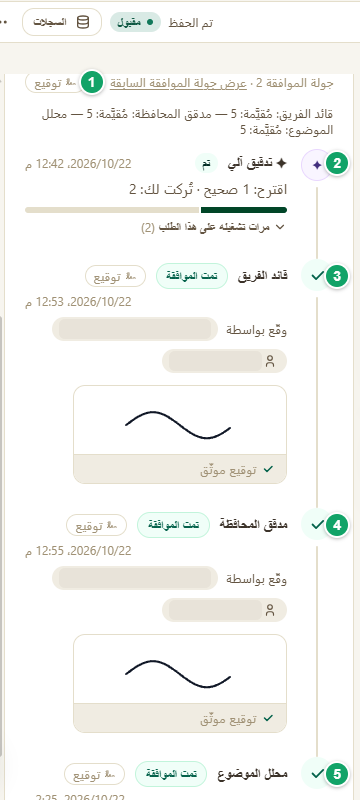
\includegraphics[width=0.45\linewidth]{assets/screens/review-chain-ar.png}
\caption{سجل المراجعة بعد اكتمال التواقيع}
\label{fig:review-chain}
\shotnote{يحفظ هذا السجل من راجع ومتى ووقّع، في كل جولة موافقة. يفيدك في إثبات أن الرقم مرّ بكل مراجعيه قبل استخدامه. أُخفيت أسماء الموقّعين. ① «جولة الموافقة 2»، و«عرض جولة الموافقة السابقة». ② «تدقيق آلي»: «اقترح: 1 صحيح · تُركت لك: 2». ③ «قائد الفريق»: «تمت الموافقة»، و«توقيع موثّق». ④ «مدقق المحافظة». ⑤ «محلل الموضوع».}
\end{figure}

\textbf{ماذا يتغير بعد الاعتماد؟} تصبح الوحدة «مقبولة» في صفحة الحزمة. وعندما تُقبل كل وحدات المنشأة، يصبح التكليف «معتمدة»، ويصبح سجل الجولة «معتمد» بتاريخ الاعتماد. وتُكتب القيم المربوطة في «السجلات» كما ضبطناها في الفصل الرابع. نقرأ هذه النتائج في الفصل~\ref{ch:08-results}.

\begin{table}[H]
\centering
\caption{مشكلات المراجعة وحلولها}
\label{tab:review-problems}
\begin{tabularx}{\linewidth}{Y Y}
\rcHeaderRow
\thh{ما الذي لاحظته؟} & \thh{ماذا تفعل؟}\\
لا أرى الطلب في «بانتظارك» & هل وقّعت المرحلة السابقة؟ فخالد لا يرى الطلب قبل ليلى.\\
زر «موافقة» معطّل & غيّر تقييم الإجابة المؤشَّر عليها، أو اختر «إعادة للتصحيح».\\
لا يكتمل التوقيع & أنشئ مفتاح التوقيع من «إدارة التوقيع»، واختر ملفه عند التوقيع.\\
لا تقبل الصفحة «توقّع وتراجع» & ضع أسئلتها داخل قسم.\\
الإجابة المرسلة لم تدخل المراجعة & بدأت قبل نشر الخطوة، فبقيت على الإصدار القديم.\\
\end{tabularx}
\end{table}

\begin{rcnote}[تطبيق المثال]
توقّع ليلى، فتصبح الإجابة «المرحلة 3 من 4» عند خالد. يقيّم خالد الإجابات الخمس ويوقّع، ثم توقّع رنا التوقيع الأخير. تصبح «بيانات التشغيل» «مقبول». وتمر «متابعة الاحتياج» بليلى ثم رنا. فتعرض الحزمة «2 من 2 أُرسلت · 2 مقبولة»، ويصبح التكليف «معتمدة».
\end{rcnote}

\begin{rcchecklist}[بعد اكتمال المراجعة]
\begin{checklist}
\item خطوة الموافقة تعمل في «مُرسل»، ومراحلها: تدقيق آلي، ثم ليلى، ثم خالد، ثم رنا.
\item الصفحتان «توقّع وتراجع»، وأسئلة كل صفحة داخل قسم.
\item أعادت ليلى «سبب التوقف» بملاحظة واضحة، وصححه عمر.
\item وقّع الثلاثة في «جولة الموافقة 2»، وصارت الإجابة «مقبول».
\item التكليف «معتمدة»، وسجل الجولة «معتمد».
\end{checklist}
\end{rcchecklist}

صارت بيانات مصنع الأفق معتمدة. في الفصل~\ref{ch:08-results} نقرأ تقدم المسح ونتائجه.
